\section*{The dispersion relation of disks}\label{sec:dispersion}

\subsection*{The dispersion relation in Keplerian disks.}
To study the oscillations generated in the disk
we use the dispersion relation derived in the appendix.
Which is given by the expression:

\begin{equation}\label{eq:dispersion}
(\tilde{\omega}^2 - \kappa^2)(\tilde{\omega}^2 - n\Omega_k^2) =
\tilde{\omega}^2 c_s^2 k_r^2
\end{equation}

Where $\tilde{omega}$ is related with number of arms of the
perturbation as:

\begin{equation}
\tilde{\omega} = \omega - m\Omega
\end{equation}

And the epicyclic frequency is:

\begin{equation}
\kappa^2 = 2\Omega \left( 2\Omega + r \dfrac{d\Omega}{dr}  \right)
\end{equation}

To understand the physical meaning of this dispersion relation lets
study some limiting cases. First if the oscillations take place in 
the plane of the disk $n=0$ the relation Eq.\ref{eq:dispersion}
reduces to:

\begin{equation}\label{eq:disp1}
\tilde{\omega}^2 = \kappa^2 + k_r^2 c_s^2
\end{equation}

This condition is known as the \textbf{inertial-acoustic} waves,
and corresponds to the oscillations of a fluid element that is
displaced in the radial direction. The oscillations arise due to the
resorting force due to rotation that brings back the fluid to the
initial position.
The oscillation frequency is the epicyclic frequency $\kappa(r)$ first
term in the right part of equation \ref{eq:disp1}. While the second
term corresponds to acoustic oscillations due to the restoring force
from compressible fluids.

If we consider oscillations in the vertical direction ($k_r=0$) the
dispersion relation Eq.\ref{eq:disp1} reduces to the following
expressions:

\begin{equation}
\tilde{\omega}^2 = \kappa^2
\end{equation}

\begin{equation}
\tilde{\omega}^2 = n \Omega_K^2
\end{equation}

The las expression corresponds to vertical oscillations in the disk, due to a
perturbation of a fluid element in the vertical direction. The
vertical component of the gravitational force in the restoring force
that returns the fluid element to the plane of the disk. The frequency
of this oscillations is represented by $\Omega_K$.


The above two limiting cases are present at the same time in disks.
The two oscillations are coupled in the form $(\tilde{\omega}^2 -
\kappa^2)(\tilde{\omega}^2 - n\Omega_k^2)$ in the dispersion relation
Eq.\ref{eq:dispersion}. Vertical oscillations induce perturbations
in the radial direction and radial oscillations induce vertical
oscillations due to inhomogeneities in the disk. The
coupling is stronger when the radial wavelength is shorter and the
acoustic speed is faster.

The dispersion relation Eq.\ref{eq:dispersion} is quadratic for
$\tilde{\omega}^2$ and the solutions are:

\begin{equation}\label{eq:sol}
\tilde{\omega}^2 = \dfrac{(n\Omega_k^2 + \kappa^2 + c_s^2 K_r^2) \pm
\sqrt{( - 4\kappa^2n\Omega_k^2)}}{2}
\end{equation}

The modes with higher $\tilde{\omega}$ are called \textbf{p-modes} 
while the solutions with lower $\tilde{\omega}$ are called
\textbf{g-modes}, this terminology is used in analogy to the one used
in stellar oscillations. It is important to recognize that in the case
of oscillations in the plane of the disk $n=0$ there are only p-modes.
In Fig.\ref{fig:gpmodes} the g-mode and p-mode are illustrated for two
cases. The left panel where $n=0$, $m=0$ shows the p-mode, in this case
$\omega^2 > \kappa^2$ in the dispersion relation because
$k_r \geq 0$. The p-mode wave propagates until it reaches the
surface of the object at $r_b$ or the epicyclic frequency $\kappa$
where it is reflected. The right panel shows the case $n=2$, $m=0$
the p-mode will be greater than $\sqrt{2}\Omega_K$ while the g-mode in
this case is lower than $\kappa$.

\begin{figure}\label{fig:gpmodes}
\centering
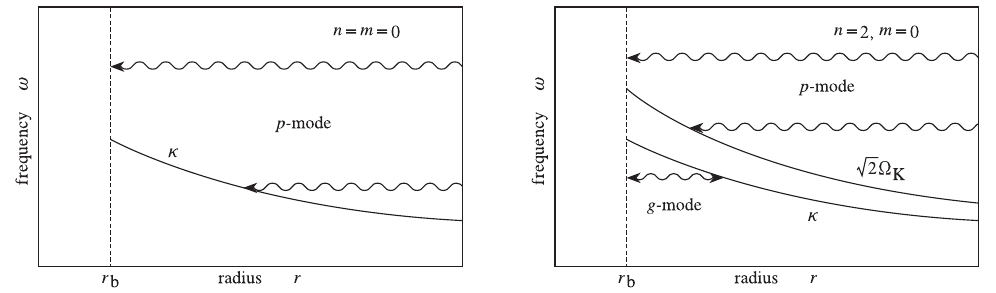
\includegraphics[scale=0.5]{waves.png}
\caption{Illustration of the p-modes and g-modes for two cases.
$n=m=0$ and $n=2$(left), $m=0$ (right).}
\end{figure}



\subsection*{The dispersion relation in the General Relativistic
regime.}

When the central object is very massive, general relativistic effects
become relevant, therefore the dispersion relation
Eq.\ref{eq:dispersion} is not longer valid in this regime. The radial
dependence of the epicyclic frequency is going to different from the
one considered in the Keplerian case, it has to be derived from the
Kerr metric which is the metric that describes massive objects such as
neutron stars and black holes. The epicyclic frequency is given by
\verb+\citep{Olkazaki87}+.

\begin{equation}
\kappa^2 = \dfrac{GM}{r^3}\left( 1 + \dfrac{a}{\hat{r}^{3/2}}
\right)^{-2} \left(1 - \dfrac{6}{\hat{r}} + \dfrac{8a}{\hat{r}^{3/2}}
- \dfrac{3a^2}{\hat{r}^2}  \right)
\end{equation}

Where $a$ is a dimensionless parameter specifying the amount of
angular momentum of the central object if $a=0$ the object is rotating
and if $a=1$ the central object have the maximum rotation. And
$\hat{r}$ is a dimensionless radius defined as:

\begin{equation}
\hat{r} = \dfrac{r}{GM/c^2}
\end{equation}

The frequency of vertical oscillations $\Omega_{\bot}$ is also modified
if the central object is rotating, $\Omega_{\bot}$ is given by:

\begin{equation}
\Omega_{\bot}^2 = \Omega_{K}^2 \left(1 - \dfrac{4a}{\hat{r}^{3/2} +
\dfrac{3a^2}{\hat{r}^2}} \right)
\end{equation}

Where $\Omega_K$ is the Keplerian vertical frequency that in the
relativistic case is also modified as:

\begin{equation}
\Omega_K^2 = \dfrac{GM}{r^3} \left[ 1 + \dfrac{a}{(8
\hat{r}^3)^{1/2}}\right]^{-1}
\end{equation}

Note that in the Keplerian case $\Omega_{\bot} = \Omega{K}$. The
redial dependence of these quantities is shown in Fig.\ref{fig:rela}
for a spin parameter of $a=0.998$. Note that $\kappa$ have a maximum
and then decrease very fast, this behavior would be the cause of
trapped waves. In the case of $a=0$ $\Omega_{\bot} = \Omega_K$.

The dispersion relation for the general relativistic is given by:

\begin{equation}\label{reladispersion}
(\tilde{\omega}^2 - \kappa^2)(\tilde{\omega}^2 - n\Omega_{\bot}^2 ) =
\tilde{\omega}^2 c_s^2 k_r^2
\end{equation}

Which is not very different from the Keplerian dispersion relation,
however the derivation of this is based in physical arguments. More
rigorous derivations have been made by
\verb+\citep{Ipser,Perez,Silbergleit}+.

\begin{figure}\label{fig:rela}
\centering
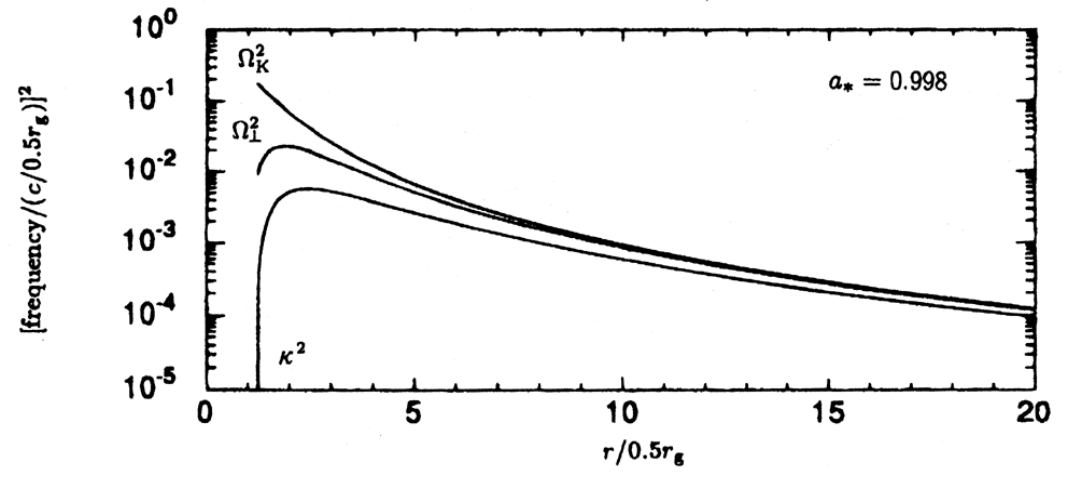
\includegraphics[scale=0.3]{relativsitc.png}
\end{figure}

